% Source problem: 2013ap_exam.pdf, PDF pp. 4--5.
\documentclass[11pt,a4paper]{article}
\usepackage[margin=22mm]{geometry}
\usepackage{fontspec}
\usepackage{xeCJK}
\setCJKmainfont{HaranoAjiMincho-Regular.otf}
\setCJKsansfont{HaranoAjiGothic-Medium.otf}
\usepackage{amsmath,amssymb}
\usepackage{tikz}
\setlength{\parindent}{1em}
\setlength{\parskip}{0.35em}
\title{物理工学専攻 院試解答集\\2013年 物理学I 第2問}
\author{政岡凜太郎}
\date{}
\begin{document}
\maketitle

以下、真空中を考える。

\section*{[1] 電流が作る磁場}
\subsection*{[1.1] 円環電流}
円環の各電流要素から軸上の点までの距離は $\sqrt{a^2+z^2}$ である。対称性により横成分は相殺し、軸成分だけが加わる。Biot--Savart則から
\begin{align}
 B_z(0,0,z)
 &=\frac{\mu_0 I}{4\pi}\int_0^{2\pi}
       \frac{a^2\,d\theta}{(a^2+z^2)^{3/2}}
 =\boxed{\frac{\mu_0 I a^2}{2(a^2+z^2)^{3/2}}}.
\end{align}
図1の電流方向へ右手の指を曲げると、親指が $+z$ を向く。

\subsection*{[1.2] 有限長ソレノイドの中心磁場}
巻数が長さ方向に一様に分布するとし、単位長さあたりの巻数を $n=N/l$ とする。軸方向位置 $z'$ にある幅 $dz'$ の巻線は $n\,dz'$ 回の円電流に相当する。その中心への寄与を[1.1]に重ねると
\begin{align}
 B_z(0)
 &=\frac{\mu_0 n I a^2}{2}
   \int_{-l/2}^{l/2}\frac{dz'}{(a^2+z'^2)^{3/2}}\\
 &=\frac{\mu_0 N I}{2\sqrt{a^2+(l/2)^2}}
 =\boxed{\frac{\mu_0 N I}{\sqrt{l^2+4a^2}}}.
\end{align}
中心磁場はソレノイド軸方向である。有限長の結果であり、$l\gg a$ の極限では $B_z(0)\simeq\mu_0NI/l$ となる。

\subsection*{[1.3] 自己インダクタンス}
自己インダクタンスの計算では $l\gg a$ とし、内部磁場を一様とみなす。各巻線を貫く磁束は
\begin{equation}
 \Phi=B\pi a^2\simeq\frac{\mu_0NI}{l}\pi a^2.
\end{equation}
全磁束鎖交数は $N\Phi=LI$ だから
\begin{equation}
 \boxed{L=\frac{N\Phi}{I}=\frac{\mu_0N^2\pi a^2}{l}.}
\end{equation}

\section*{[2] 交流コンデンサー間の電磁場}
極板間隔 $d\ll b$ として端効果を無視し、極板半径が交流の波長に比べて十分小さい準静的近似を用いる。
その条件は $\omega_0 b\sqrt{\mu_0\varepsilon_0}\ll1$ であり、電磁波の伝播に伴う電場の空間変化を無視する。
極板間の電場を $+z$ 方向に正として選ぶと
\begin{equation}
 \boldsymbol E(t)=\frac{v_0}{d}\sin(\omega_0t)\,\boldsymbol e_z.
\end{equation}
端効果を無視し、半径 $r<b$ の円周を囲む積分路にMaxwell--Amp\`ere則を適用する。電束は $\pi r^2E_z$ なので
\begin{equation}
 2\pi r B_\phi=\mu_0\varepsilon_0\frac{d}{dt}(\pi r^2E_z),
 \qquad
 \boxed{\boldsymbol B(r,t)=\frac{\mu_0\varepsilon_0\omega_0v_0r}{2d}
     \cos(\omega_0t)\,\boldsymbol e_\phi.}
\end{equation}
$\cos(\omega_0t)>0$ のとき $\boldsymbol B$ は $+z$ 軸から見て反時計回り、$\cos(\omega_0t)<0$ では時計回りである。電場の時間変化に対する右ねじの向きであり、$\cos=0$ では磁場は瞬間的にゼロとなる。

\section*{[3] LC回路}
\subsection*{[3.1] 電流の時間変化}
最初にコンデンサーに蓄えられた電荷を $q(0)=CV$ とする。$i$ の正方向をコンデンサーが放電するときの向きに取れば $i=-\dot q$ で、初期電流は $i(0)=0$ である。回路の電圧則は
\begin{equation}
 \frac{q}{C}=L\frac{di}{dt}=-L\frac{d^2q}{dt^2},
 \qquad \ddot q+\frac{1}{LC}q=0.
\end{equation}
角振動数 $\omega=1/\sqrt{LC}$ の解は
\begin{equation}
 \boxed{q(t)=CV\cos(\omega t),\qquad
 i(t)=-\dot q=CV\omega\sin(\omega t).}
\end{equation}
電流は最初ゼロから増え、コンデンサーが空になる $t=\pi/(2\omega)$ で最大となる。

\subsection*{[3.2] 電場・磁場エネルギー}
コンデンサーとソレノイドのエネルギーは
\begin{equation}
 U_C(t)=\frac{q^2}{2C}=E_0\cos^2(\omega t),\qquad
 U_L(t)=\frac12Li^2=E_0\sin^2(\omega t),\qquad E_0=\frac12CV^2.
\end{equation}
したがって $U_C+U_L=E_0$ は一定である。$t=0$ では全エネルギーが電場にあり、$t=\pi/(2\omega)$ では磁場に移り、$t=\pi/\omega$ では再び電場に戻る。この交換が繰り返される。横軸を $\omega t$、縦軸を $U/E_0$ とした同一図に示す。
\begin{center}
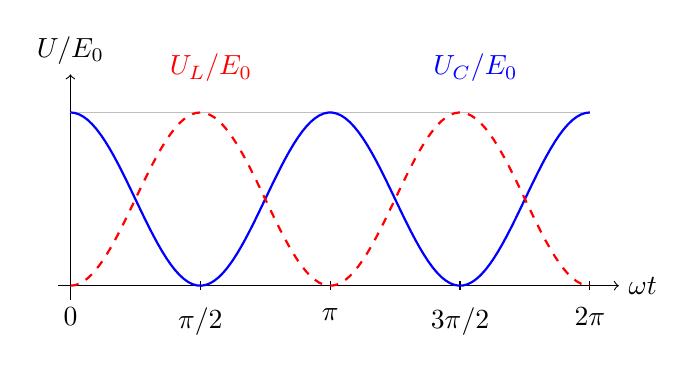
\begin{tikzpicture}[x=1.05cm,y=2.2cm]
 \pgfmathsetmacro{\period}{2*pi}
 \pgfmathsetmacro{\axisEnd}{\period+0.35}
 \draw[->] (-0.15,0) -- (\axisEnd,0) node[right] {$\omega t$};
 \draw[->] (0,-0.08) -- (0,1.22) node[above] {$U/E_0$};
 \foreach \n/\lab in {0/0,1/{\pi/2},2/{\pi},3/{3\pi/2},4/{2\pi}} {
   \pgfmathsetmacro{\tickx}{\n*pi/2}
   \draw (\tickx,0.025)--(\tickx,-0.025) node[below=3pt] {$\lab$};
 }
 \draw[gray!50] (0,1)--(\period,1);
 \draw[thick,blue,samples=120] plot[domain=0:360] ({\x*pi/180},{cos(\x)^2});
 \draw[thick,red,dashed,samples=120] plot[domain=0:360] ({\x*pi/180},{sin(\x)^2});
 \node[blue,anchor=south] at (4.9,1.12) {$U_C/E_0$};
 \node[red,anchor=south] at (1.7,1.12) {$U_L/E_0$};
\end{tikzpicture}
\end{center}

\subsection*{[3.3] 極板間隔を $2d$ にした場合}
スイッチをつなぐ前に極板を引き離す間、漏れがないため電荷 $Q=CV$ は一定である。平行板容量が $C'=C/2$ となり、電圧は $V'=Q/C'=2V$ に上がる。従って接続直後の全エネルギーと固有角振動数は
\begin{equation}
 U'_0=\frac{Q^2}{2C'}=CV^2=2E_0,
 \qquad \omega'=\frac{1}{\sqrt{LC'}}=\sqrt2\,\omega.
\end{equation}
以後 $q(0)=Q$, $i(0)=0$ なので
\begin{equation}
 U'_C(t)=2E_0\cos^2(\sqrt2\omega t),\qquad
 U'_L(t)=2E_0\sin^2(\sqrt2\omega t).
\end{equation}
同じ規格化 $U/E_0$ と横軸 $\omega t$ で描くと、エネルギー振幅が2倍、振動数が $\sqrt2$ 倍になる。
\begin{center}
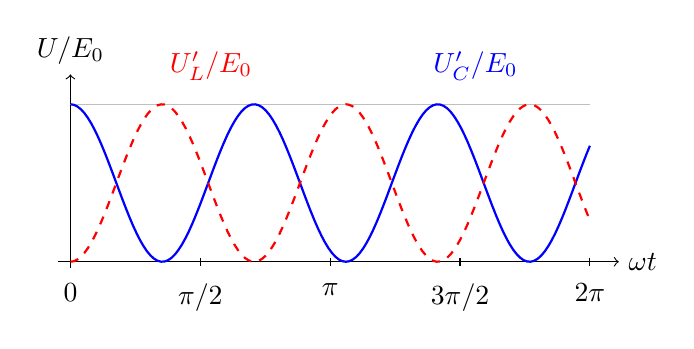
\begin{tikzpicture}[x=1.05cm,y=1.0cm]
 \pgfmathsetmacro{\period}{2*pi}
 \pgfmathsetmacro{\frequencyRatio}{sqrt(2)}
 \pgfmathsetmacro{\axisEnd}{\period+0.35}
 \draw[->] (-0.15,0) -- (\axisEnd,0) node[right] {$\omega t$};
 \draw[->] (0,-0.08) -- (0,2.38) node[above] {$U/E_0$};
 \foreach \n/\lab in {0/0,1/{\pi/2},2/{\pi},3/{3\pi/2},4/{2\pi}} {
   \pgfmathsetmacro{\tickx}{\n*pi/2}
   \draw (\tickx,0.05)--(\tickx,-0.05) node[below=3pt] {$\lab$};
 }
 \draw[gray!50] (0,2)--(\period,2);
 \draw[thick,blue,samples=150] plot[domain=0:360] ({\x*pi/180},{2*cos(\frequencyRatio*\x)^2});
 \draw[thick,red,dashed,samples=150] plot[domain=0:360] ({\x*pi/180},{2*sin(\frequencyRatio*\x)^2});
 \node[blue,anchor=south] at (4.9,2.18) {$U'_C/E_0$};
 \node[red,anchor=south] at (1.7,2.18) {$U'_L/E_0$};
\end{tikzpicture}
\end{center}
極板間隔を増すには、極板間の引力に逆らって外力が仕事をする必要がある。理想的な容量モデルで損失を無視し、極板を静止させた前後の状態を比べると、外力の仕事は電気エネルギーの増加 $U'_0-E_0=Q^2/(2C')-Q^2/(2C)=E_0$ に等しい。接続後はその増えた全エネルギーがコンデンサーとソレノイドの間を移る。

\end{document}
